Nuevas normas como, por ejemplo, las establecidas por la ITU-T, el IEC y el Instituto de Ingeniería Electrónica y Eléctrica (IEEE), han incrementado en gran medida la estandarización del diseño, la viabilidad y la seguridad de PONs; lo que brinda la oportunidad de economías escala y menores costes, no concebibles anteriormente.

Las figuras~\figref{fig:PON_Now}~y~\figref{fig:PON_Next} resumen los principales parámetros que definen esas normas.

\begin{figure}[H]
	\centering
	\includegraphics[width=0.75\textwidth]{./img/punto1/Tecnologías-PON-actualmente-implantadas.jpg}
	\caption{Tecnologías PON actualmente implantadas}
	\label{fig:PON_Now}
\end{figure}


\begin{figure}[H]
	\centering
	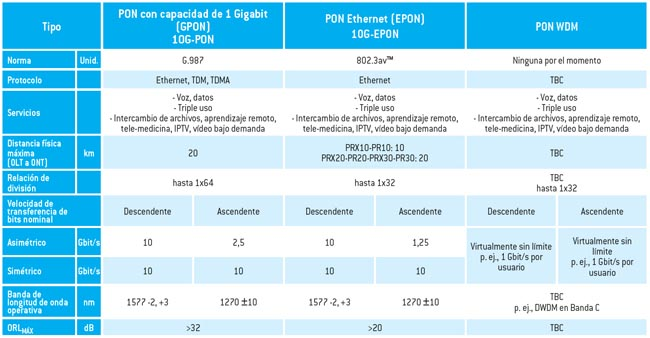
\includegraphics[width=0.75\textwidth]{./img/punto1/Tecnologías-PON-de-próxima-generación.jpg}
	\caption{Tecnologías PON de próxima generación}
	\label{fig:PON_Next}
\end{figure}